\documentclass[notes]{subfiles}
\begin{document}
	\addcontentsline{toc}{section}{1.4 - Linear Functions \& Models}
	\refstepcounter{section}
	\fancyhead[RO,LE]{\bfseries \large \nameref{cs14}} 
	\fancyhead[LO,RE]{\bfseries \currentname}
	\fancyfoot[C]{{}}
	\fancyfoot[RO,LE]{\large \thepage}	%Footer on Right \thepage is pagenumber
	\fancyfoot[LO,RE]{\large Chapter 1.4}



\section*{Linear Functions \& Models}\label{cs14}
	\subsection*{Linear Functions}
		Remember that a linear function requires two pieces of information- a starting value ($b$, the $y$-intercept), and an amount of incremental change in the independent variable ($m$, the slope of the function).  This gives us three ways to describe a linear function:\\[10pt]
		\begin{itemize}
			\item \underline{Verbally}: \showto{ins}{\fbox{A function with a constant rate of change}}\showto{st}{\\[10pt]}
			\item \underline{Graphically}: \showto{ins}{\fbox{There are images below}}\showto{st}{\\[10pt]}
			\item \underline{Algebraically}: \showto{ins}{\fbox{$f(x) = mx + b$}}\showto{st}{\\[10pt]} 
		\end{itemize}
			\vs{.25}
		\begin{question}
			Given two points $(x_1,y_1)$ and $(x_2,y_2)$, how can we find the slope of the line between them?
		\end{question}
			\vs{.5}
	\subsection*{Linear Models}
		 For our general model, $f(x) = ax + b$, we have the following characteristics:
		\begin{figure}[h!]	
			\fbox{
			\begin{minipage}{1in}
			\centering
				$\underline{a > 0}$\\
				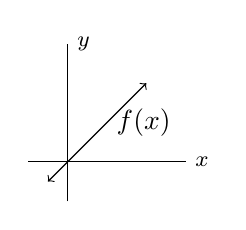
\begin{tikzpicture}[x = .5cm, y = .5cm]
				\draw (-1,0)--(3,0) node[right] {\footnotesize $x$}; %x-axis
				\draw (0,-1)--(0,3) node[right] {\footnotesize $y$}; %y-axis
				\draw[<->, smooth, samples = 10, domain = -.5:2.0] plot (\x, {\x});	
				\draw (1,1) node[right] {$f(x)$};
				\end{tikzpicture}	
			\end{minipage}
			\begin{minipage}{2in}
				\begin{itemize}
					\item $\ds \lim_{x\to\infty} f(x) =$\showto{ins}{\fbox{$\infty$}}\showto{st}{}
					\item $\ds \lim_{x\to -\infty} f(x) =$ \showto{ins}{\fbox{$-\infty$}}\showto{st}{}
					\item $f$ is always \showto{ins}{\fbox{increasing}}\showto{st}{}
					\item $f$ has no concavity
				\end{itemize}
			\end{minipage}
			}
			\fbox{
			\begin{minipage}{1in}
			\centering
				$\underline{a < 0}$\\
				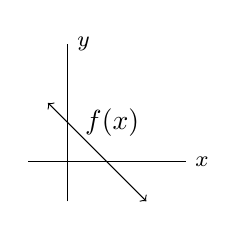
\begin{tikzpicture}[x = .5cm, y = .5cm]
					\draw (-1,0)--(3,0) node[right] {\footnotesize $x$}; %x-axis
					\draw (0,-1)--(0,3) node[right] {\footnotesize $y$}; %y-axis
					\draw[<->, smooth, samples = 10, domain = -.5:2.0] plot (\x, {-\x + 1});
					\draw (.2,1) node[right] {$f(x)$};	
				\end{tikzpicture}
				\end{minipage}
			\begin{minipage}{2in}
				\begin{itemize}
					\item $\ds \lim_{x\to\infty} f(x) =$ \showto{ins}{\fbox{$-\infty$}}\showto{st}{}
					\item $\ds \lim_{x\to -\infty} f(x) =$ \showto{ins}{\fbox{$\infty$}}\showto{st}{}
					\item $f$ is always \showto{ins}{\fbox{decreasing}}\showto{st}{}
					\item $f$ has no concavity
				\end{itemize}
			\end{minipage}
			}
	
			\fbox{
			\begin{minipage}{1in}
			\centering
				$\underline{a = 0}$\\
				\begin{tikzpicture}[x = .5cm, y = .5cm]
					\draw (-1,0)--(3,0) node[right] {\footnotesize $x$}; %x-axis
					\draw (0,-1)--(0,3) node[right] {\footnotesize $y$}; %y-axis
					\draw[<->, smooth, samples = 10, domain = -.5:3.0] plot (\x, {1});
					\draw (1.5,1) node[above] {$y = b$};
				\end{tikzpicture}
			\end{minipage}
			\begin{minipage}{1.95in}
				\begin{itemize}
					\item $\ds \lim_{x\to\infty} f(x) =$ \showto{ins}{\fbox{$b$}}\showto{st}{}
					\item $\ds \lim_{x\to -\infty} f(x) =$ \showto{ins}{\fbox{$b$}}\showto{st}{}
					\item $f$ is always \showto{ins}{\fbox{constant}}{}
					\item $f$ has no concavity
				\end{itemize}
			\end{minipage}
			}
			\fbox{
			\begin{minipage}{1in}
			\centering
				\underline{$a$ undefined}\\
				\begin{tikzpicture}[x = .5cm, y = .5cm]
					\draw (-1,0)--(3,0) node[right] {\footnotesize $x$}; %x-axis
					\draw (0,-1)--(0,3) node[right] {\footnotesize $y$}; %y-axis
					\draw[<->] (1,-.5)--(1,2.5);
					\draw (2,1) node[xshift = 5pt] {$x = b$};
				\end{tikzpicture}
			\end{minipage}
			\begin{minipage}{2in}
				\begin{itemize}
					\item $\ds \lim_{x\to\infty} f(x)=$ \showto{ins}{\fbox{DNE}}\showto{st}{}
					\item $\ds \lim_{x\to -\infty} f(x)=$ \showto{ins}{\fbox{DNE}}\showto{st}{}
					\item Neither inc. nor dec.
					\item No concavity
				\end{itemize}
			\end{minipage}
			}
		\end{figure}
		%%%In future iterations of these notes, I want to make these graphs a little bit prettier/more flexible.  I don't have time to do it right now

		For any given graph, the scales \emph{\textbf{will}} change; use algebra, don't trust your eyes.
		\newpage
		
	\subsection*{Elements of a Model}
		From now on, when we refer to a model, we are referring to a specific collection of information.  These pieces are listed below; \emph{memorize them}!  \\
		\begin{enumerate}[(1)]
			\item \fitb{Proper and consistent function notation}{$ $ \vs{.75}}
			\item \fitb{Model coefficients rounded to \textbf{three} decimal places}{$ $ \vs{.75}}
			\item \fitb{Output units}{$ $\vs{.75}}
			\item \fitb{Output description}{$ $\vs{.75}}
			\item \fitb{Input units}{$ $\vs{.75}}
			\item \fitb{Input description}{$ $\vs{.75}}
		\end{enumerate}
		\begin{ex}
			The following table gives the percentage of new companies which remained open $t$ years after beginning business.
			\begin{center} 
				{\renewcommand{\arraystretch}{1.2}
				\begin{tabular}{|l||c|c|c|c|c|c|} \hline
					\textbf{Years After Opening} & 5 & 6 & 7 & 8 & 9 & 10\\ \hline
					\textbf{Companies Still Open} (in \%) & 50 & 47 & 44 & 41 & 38 & 35\\ \hline
				\end{tabular}
				}
			\end{center}
			\begin{enumerate}[(a)]
				\item Fill in the new inputs if we align the data so that the fifth year corresponds to an input of zero.
					\begin{center} 
						{\renewcommand{\arraystretch}{1.75}
						\begin{tabular}{|l||P{.5in}|P{.5in}|P{.5in}|P{.5in}|P{.5in}|P{.5in}|} \hline
							\textbf{Years After Opening} &  &  &  &  &  & \\ \hline
							\textbf{Companies Still Open} (in \%) & 50 & 47 & 44 & 41 & 38 & 35\\ \hline
						\end{tabular}
						}
					\end{center}
				\item Use the aligned data to create a \textbf{complete} model.
					\vs{2}
			\end{enumerate}
				\newpage
		\end{ex}

		\begin{defn}[Extrapolation]
			When using a model, we say that data is \textbf{extrapolated} if we find an output value\\[15pt] \showto{ins}{\fbox{outside of the interval of the input data.}}\showto{st}{\blank{5}.}

		\end{defn}
			\vspace{.25in}
		\begin{defn}[Interpolation]
			When using a model, we say that data is \textbf{interpolated} if we find an output value\\[15pt] \showto{ins}{\fbox{outside of the interval of the input data}}\showto{st}{\blank{5}}.
		\end{defn}
		\begin{ex}
			In the example above, predict the number of companies open in the twelfth year of operation.  Is this extrapolation or interpolation?
		\end{ex}
			\vs{.25}
		\begin{ex}
			Do the same, but after 8.5 years after opening.  Is this extrapolation or interpolation?
		\end{ex}
			\vs{.25}
		\begin{ex}
			The amount of electricity sold by a power company in year $x$ is given below.
			\begin{center}
				{\renewcommand{\arraystretch}{1.2}
				\begin{tabular}{|l||c|c|c|c|c|c|} \hline
					\textbf{Year} & 2003 & 2004 & 2005 & 2006 & 2007 & 2008 \\ \hline
					\textbf{Retail Sales} (in quadrillion kWh) & 1.2 & 1.23 & 1.27 & 1.3 & 1.33 & 1.35\\ \hline
				\end{tabular}
				}
			\end{center}
			\begin{enumerate}[(a)]
				\item Find a \textbf{complete} linear model to fit the data.  
					\vs{1}
				\item Write an interpretation the slope of the linear model.
					\vs{1}
				\item When did retail sales first exceed 1.4 quadrillion kWh?  Is this interpolation or extrapolation?
					\vs{.5}
			\end{enumerate}
		\end{ex}
			\newpage

	\subsection*{Data Alignment}
		When using an input value of years, alignment should (usually) happen so that the first year given corresponds to an input of zero.

		\begin{ex}
			Find the \textbf{complete} linear model to fit the data of the previous example, aligning the input so that the year 2003 corresponds to an input of zero.
		\end{ex}
			\vs{1}
			
			
	\subsection*{Numerical Considerations}
		Since numerical approximations can vary, we will use the following guidelines:
		\begin{enumerate}[(1)]
			\item Use common sense; if a model outputs something like ``2.5 people'', we would round to 3 people.
			\item The accuracy of the output \textbf{must} be the same as the original model's accuracy.
			\item All answers \textbf{must} have proper units; answers without labels are useless.
			\item If arriving at your answer requires multiple steps, \textbf{do not} round until the \emph{final} answer.
		\end{enumerate}
			\vspace{.1in}
		\begin{ex}
			The world's daily demand of oil was recorded in various years, and is listed below.
			\begin{center}
				{\renewcommand{\arraystretch}{1.2}
				\begin{tabular}{|l||c|c|c|c|c|c|} \hline
					\textbf{Year} & 2004  & 2005 & 2006 & 2007 & 2008 & 2009 \\ \hline
					\textbf{Oil Demand} (in million barrels) & 82.327 & 83.652 & 84.622 & 85.385 & 86.384 & 87.698\\ \hline
				\end{tabular}	
				}
			\end{center}
			\begin{enumerate}[(a)]
				\item Based on the scatterplot, why is a linear model best?
					\vs{.5}
				\item Align the data so that the year 2000 corresponds to an input of 0, and find the \textbf{complete} linear model.
					\vs{1}
				\item Estimate the demand in the year 2015.
					\vs{.5}
			\end{enumerate}
		\end{ex}
			\newpage

		\begin{ex} Expenditure on pets in the United States was recorded over the span of several years, and is recorded in the table below.
			\begin{center}
				{\renewcommand{\arraystretch}{1.2}
				\begin{tabular}{|P{1in}||c|c|c|c|c|c|c|c|c|c|c|}\hline
					\textbf{Year} & 1994 & 1996 & 1998 & 2001 & 2002 & 2003 & 2004 & 2005 & 2006 & 2007 & 2008 \\ \hline
					\textbf{Expenditure} (billion USD) & 17 & 21 & 23 & 28.5 & 29.5 & 32.4 & 34.4 & 36.3 & 38.5 & 41.2 & 43.4\\ \hline
				\end{tabular}
				}
			\end{center}
			\begin{enumerate}[(a)]
				\item Align the data so that the year 1994 corresponds to an input of zero, and find the \textbf{complete} linear model.
					\vs{1}
				\item Use the model to estimate the expenditure in the year 2013.
					\vs{.5}
			\end{enumerate}
		\end{ex}

		\begin{ex}
			The number of successful tax audits performed by a company between 2000 and 2006 can be modeled by $A(t) = -83.9t + 1063$ audits, where $t$ is the number of years since 2000.  
			\begin{enumerate}[(a)]
				\item Give the rate of change of $A$. Include units.
					\vs{.5}
				\item Evaluate $A(0)$.  Write a sentence interpreting your answer.
					\vs{.5}
				\item Find the number of successful audits in 2005.  Is this interpolation or extrapolation?
					\vs{.5}
				\item Find the number of successful audits in 2010.  is this interpolation or extrapolation?
					\vs{.5}
			\end{enumerate}
		\end{ex}
			\newpage

		\begin{ex}
			The population of a town in selected years is given below.
			\begin{center}
				{\renewcommand{\arraystretch}{1.2}
				\begin{tabular}{|c||c|c|c|c|c|c|}\hline
					\textbf{Year} & 2005 & 2006 & 2007 & 2008 & 2009 & 2010\\ \hline
					\textbf{Population} (in thousands) & 125.2 & 128.7 & 132.4 & 136.0 & 139.8 & 143.6\\ \hline
				\end{tabular}
				}
			\end{center}
			\begin{enumerate}[(a)]
				\item Find a \textbf{complete} model for the population $P$ of the town in year $y$.
					\vs{1}
				\item According to your model, what is the constant rate of change of the population of the town?
					\vs{.5}
				\item Use your model to predict the population of the town in 2015.
					\vs{.5}
			\end{enumerate}	
		\end{ex}

		\begin{ex}
			Honda engineers are designing a new car, and are measuring the distance it takes the car to come to a complete stop on dry pavement.  Their measurements are given below.
			\begin{center}
				{\renewcommand{\arraystretch}{1.2}
				\begin{tabular}{|c|c|c|c|c|c|}\hline
					\textbf{Speed} (mph) & 55 & 60 & 65 & 70 & 75 \\ \hline				
					\textbf{Distance} (ft) & 77.6 & 131.4 & 186.3 & 236.7 & 289.3\\ \hline
				\end{tabular}
				}
			\end{center}
			\begin{enumerate}[(a)]
				\item Find a \textbf{complete} model for the braking distance of the car.
					\vs{1}
				\item Use your model to find the braking distance needed when the car is traveling at 77 miles per hour; write your answer using function notation.
					\vs{.5}
				\item Find another \textbf{complete} model, aligning the data so that a speed of 50 mph corresponds to an input of 0.
					\vs{1}
				\item Repeat part (b).
					\vs{.5}
				\item How fast is the car traveling if it requires 156 ft to come to a complete stop?
					\vs{.5}
			\end{enumerate}
		\end{ex}
	\clearpage	
\end{document}